% ==============================================================================
% SLIDE BÁO CÁO BÀI TẬP LỚN - ĐẠI HỌC XÂY DỰNG HÀ NỘI (HUCE)
% ĐỀ TÀI: ỨNG DỤNG HỌC MÁY TRONG PHÁT HIỆN BOTNET TỪ LƯU LƯỢNG MẠNG
% ==============================================================================
\documentclass[lualatex,10pt,unknownkeysallowed]{beamer}

% Kiểm tra gói style arpa-fvg của template (nếu có thì nạp, nếu không thì dùng chuẩn HUCE)
\IfFileExists{style/arpafvg.sty}{
  \usepackage{style/arpafvg}
}{
  \usetheme{Madrid}
  \usecolortheme{whale}
}

% Hỗ trợ tiếng Việt cho LuaLaTeX / XeLaTeX hoặc pdfLaTeX
\usepackage{iftex}
\ifPDFTeX
  \usepackage[utf8]{inputenc}
  \usepackage[vietnamese]{babel}
\else
  \usepackage{fontspec}
\fi

\usepackage{graphicx}
\usepackage{booktabs}
\usepackage{hyperref}
\usepackage{color, colortbl}
\usepackage{tikz}
\usetikzlibrary{positioning, arrows.meta}

% Định nghĩa màu sắc thương hiệu Đại học Xây dựng Hà Nội (HUCE Navy Blue)
\definecolor{HuceBlue}{RGB}{0, 43, 91}
\definecolor{HuceDarkBlue}{RGB}{0, 28, 60}
\definecolor{HuceAccent}{RGB}{200, 35, 51}
\definecolor{LightGray}{gray}{0.95}

\setbeamercolor{palette primary}{bg=HuceBlue,fg=white}
\setbeamercolor{palette secondary}{bg=HuceDarkBlue,fg=white}
\setbeamercolor{palette tertiary}{bg=HuceBlue,fg=white}
\setbeamercolor{structure}{fg=HuceBlue}
\setbeamercolor{title}{bg=HuceBlue,fg=white}
\setbeamercolor{frametitle}{bg=HuceBlue,fg=white}
\setbeamercolor{block title}{bg=HuceBlue,fg=white}
\setbeamercolor{block body}{bg=LightGray,fg=black}

\graphicspath{{./}{output_charts/}}

% ------------------------------------------------------------------------------
% THÔNG TIN ĐỀ TÀI & TÁC GIẢ
% ------------------------------------------------------------------------------
\title[\textbf{Phát hiện Botnet bằng ML}]{\textbf{ỨNG DỤNG HỌC MÁY TRONG PHÁT HIỆN BOTNET TỪ LƯU LƯỢNG MẠNG}}
\subtitle{Báo cáo Bài tập lớn môn An toàn và Bảo mật thông tin}
\author[\textbf{Nhóm sinh viên}]{
  \textbf{Giảng viên hướng dẫn:} ThS. Nguyễn Việt Nhật \\[0.25cm]
  \textbf{Sinh viên thực hiện:} \\[0.1cm]
  \footnotesize
  \begin{tabular}{ll}
    Nguyễn Bá Hùng (0368269) & Nguyễn Duy Hùng (0368369) \\
    Lê Quang Huy (0368469)   & Ngô Xuân Trung (0373569) \\
    \multicolumn{2}{c}{Bùi Đức Thắng (0373069)}
  \end{tabular}
}
\institute[ĐH Xây Dựng]{\textbf{TRƯỜNG ĐẠI HỌC XÂY DỰNG HÀ NỘI (HUCE)} \\ KHOA CÔNG NGHỆ THÔNG TIN}
\date[\today]{\today}

\begin{document}

% SLIDE 1: TRANG TIÊU ĐỀ
\begin{frame}[plain]
  \vspace{-0.3cm}
  \begin{center}
    \IfFileExists{banner_huce.png}{
      % Nếu bạn dùng trực tiếp ảnh banner xanh
      
\includegraphics[height=1.15cm]{banner_huce.png}
    }{
      % Ghép logo và chữ bằng LaTeX thuần
      \begin{tabular}{c@{\hspace{0.35cm}}l}
        \IfFileExists{logo_huce.png}{
          \raisebox{-0.38\height}{
\includegraphics[height=1.25cm]{logo_huce.png}}
        }{} &
        \begin{tabular}{@{}l@{}}
          {\large \textbf{\color{HuceBlue} TRƯỜNG ĐẠI HỌC XÂY DỰNG HÀ NỘI}} \\[3pt]
          {\footnotesize \textbf{\color{HuceDarkBlue} Hanoi University of Civil Engineering}}
        \end{tabular}
      \end{tabular}
    }
  \end{center}
  \vspace{-0.2cm}
  \titlepage
\end{frame}

% SLIDE 2: TÍNH CẤP THIẾT & THÁCH THỨC
\begin{frame}{1. Đặt vấn đề \& Thách thức trong phát hiện Botnet}
  \begin{columns}[T]
    \begin{column}{0.48\textwidth}
      \begin{block}{\textbf{Mối đe dọa từ Botnet}}
        \begin{itemize}
          \item Là mạng lưới các thiết bị bị xâm nhập (Zombies/Bots) dưới quyền điều khiển của Hacker qua máy chủ C2.
          \item Vũ khí hàng đầu thực hiện: Tấn công từ chối dịch vụ (DDoS), phát tán mã độc, đào tiền ảo, gián điệp.
        \end{itemize}
      \end{block}
    \end{column}
    \begin{column}{0.48\textwidth}
      \begin{alertblock}{\textbf{Hạn chế của IDS truyền thống}}
        \begin{itemize}
          \item \textbf{Dựa trên chữ ký (Snort/Suricata):} Bất lực trước biến thể mới (Zero-day).
          \item \textbf{Mã hóa lưu lượng (HTTPS/TLS):} Chiếm $>90\%$ lưu lượng Internet, khiến việc soi nội dung gói tin (DPI) thất bại hoàn toàn.
        \end{itemize}
      \end{alertblock}
    \end{column}
  \end{columns}

  \vspace{0.3cm}
  \begin{exampleblock}{\textbf{Hướng tiếp cận của đề tài: Phân tích luồng (Flow-based ML)}}
    Không cần giải mã nội dung gói tin; tập trung học các \textbf{đặc trưng hành vi thống kê của luồng mạng} (chu kỳ kết nối, cờ TCP, tỷ lệ gửi/nhận, kích thước luồng).
  \end{exampleblock}
\end{frame}

% SLIDE 3: KIẾN TRÚC PIPELINE
\begin{frame}{2. Kiến trúc Pipeline hệ thống đề xuất}
  \begin{columns}[c]
    % Cột 1: Sơ đồ dòng chảy dọc bằng tọa độ cố định (Không bao giờ bị lỗi đè chữ)
    \begin{column}{0.44\textwidth}
      \centering
      \begin{tikzpicture}[
        box/.style={
          rectangle, 
          draw=HuceBlue, 
          thick, 
          rounded corners=3pt,
          fill=LightGray, 
          text centered, 
          minimum height=0.65cm, 
          text width=4.2cm, 
          font=\scriptsize\bfseries
        }
      ]
        \node (pcap)  at (0, 0)    [box] {1. Lưu lượng mạng PCAP};
        \node (flow)  at (0, -1.0) [box] {2. Bóc tách luồng (CICFlowMeter)};
        \node (prep)  at (0, -2.0) [box] {3. Tiền xử lý (57 đặc trưng)};
        \node (ml)    at (0, -3.0) [box] {4. Phân loại ML (Random Forest)};
        \node (alert) at (0, -4.0) [box, fill=HuceBlue, text=white] {5. Cảnh báo thời gian thực ($< 2$ms)};

        \draw[->, very thick, HuceAccent] (pcap) -- (flow);
        \draw[->, very thick, HuceAccent] (flow) -- (prep);
        \draw[->, very thick, HuceAccent] (prep) -- (ml);
        \draw[->, very thick, HuceAccent] (ml) -- (alert);
      \end{tikzpicture}
    \end{column}

    % Cột 2: Diễn giải chi tiết
    \begin{column}{0.54\textwidth}
      \begin{block}{\textbf{Trích xuất Luồng hai chiều}}
        \footnotesize
        Gom các gói tin theo ngũ bộ (5-tuple: $IP_{src}, IP_{dst}, Port_{src}, Port_{dst}, Protocol$).
      \end{block}

      \vspace{0.15cm}
      \begin{block}{\textbf{Không gian 57 đặc trưng}}
        \footnotesize
        Tính toán các chỉ số thống kê về thời gian luồng, khoảng cách giữa các gói (IAT), cờ TCP và chu kỳ nghỉ (\texttt{Idle}).
      \end{block}

      \vspace{0.15cm}
      \begin{block}{\textbf{Suy diễn thời gian thực}}
        \footnotesize
        Mô hình Random Forest phân loại với độ trễ cực thấp ($< 2$ms/flow), phù hợp tích hợp vào Router/Firewall.
      \end{block}
    \end{column}
  \end{columns}
\end{frame}

% SLIDE 4: BỘ DỮ LIỆU THỰC NGHIỆM CTU-13
\begin{frame}{3. Dữ liệu thực nghiệm chuẩn quốc tế: CTU-13}
  \begin{columns}[c]
    \begin{column}{0.55\textwidth}
      \begin{itemize}
        \item \textbf{Nguồn gốc:} Thu thập bởi \textbf{Stratosphere Laboratory} (Đại học Kỹ thuật Séc - CTU Prague) – nhóm tác giả hệ thống IDS nổi tiếng \textbf{Slips}.
        \item \textbf{Kịch bản đa dạng:} Thu giữ lưu lượng thực tế của 13 kịch bản mã độc (Neris, Rbot, Virut,...) pha trộn lưu lượng người dùng bình thường.
        \item \textbf{Quy mô mẫu thực nghiệm:}
        \begin{itemize}
          \item \textbf{Tổng số luồng:} 92,212 flows.
          \item \textbf{Botnet Attack (Label = 1):} 38,898 flows ($42.2\%$).
          \item \textbf{Normal Traffic (Label = 0):} 53,314 flows ($57.8\%$).
        \end{itemize}
        \item \textbf{Phân chia kiểm thử:} 80\% Train (73,769 mẫu) và 20\% Test độc lập (18,443 mẫu) với cơ chế \textit{Stratified Split}.
      \end{itemize}
    \end{column}
    \begin{column}{0.42\textwidth}
      \begin{block}{\textbf{Đặc thù bộ dữ liệu}}
        \centering
        \textbf{Cân bằng nhãn lý tưởng}\\
        $42.2\%$ Botnet vs $57.8\%$ Normal\\
        \vspace{0.3cm}
        Tránh hiện tượng mô hình bị lệch nhãn (Imbalanced Data), bảo đảm độ tin cậy của chỉ số Precision/Recall.
      \end{block}
    \end{column}
  \end{columns}
\end{frame}

% SLIDE 5: BẢN CHẤT KHÁC BIỆT GIỮA BOTNET VÀ NORMAL
\begin{frame}{4. Phân tích hành vi: Điểm khác biệt mấu chốt}
  \begin{table}[h]
    \centering
    \footnotesize
    \begin{tabular}{p{3.2cm} p{3.2cm} p{3.4cm}}
      \toprule
      \textbf{Đặc trưng} & \textbf{Lưu lượng thường (Normal)} & \textbf{Mã độc Botnet (Attack)} \\
      \midrule
      \textbf{Chu kỳ nghỉ (\texttt{Idle Max})} & Ngẫu hứng, thay đổi tự nhiên theo con người. & \textbf{Đều đặn có chu kỳ} (Beaconing C2 gửi gói tin giữ kết nối). \\
      \midrule
      \textbf{Tỷ lệ Gửi / Nhận (\texttt{Tot Fwd} vs \texttt{Bwd})} & Nhận về nhiều hơn gửi (\texttt{Tot Bwd} trung bình 15.7 pkts). & \textbf{Gửi nhiều hơn nhận} (\texttt{Tot Fwd} 13.6 pkts, quét cổng/phát tán). \\
      \midrule
      \textbf{Cờ kết nối (\texttt{SYN Flag Cnt})} & Tỷ lệ thấp (trung bình 15.8\%). & \textbf{Tăng vọt 53.5\%} (quét mạng Reconnaissance). \\
      \midrule
      \textbf{Dung lượng phản hồi (\texttt{TotLen Bwd Pkts})} & Lớn, đa dạng (tải trang web, tài liệu). & \textbf{Siêu nhỏ} (chỉ vài byte mã lệnh C2: Ping/Sleep/DDoS). \\
      \bottomrule
    \end{tabular}
  \end{table}
\end{frame}

% SLIDE 6: KẾT QUẢ SO SÁNH CÁC MÔ HÌNH
\begin{frame}{5. Kết quả thực nghiệm \& So sánh hiệu năng}
  \begin{table}[h]
    \centering
    \scriptsize
    \begin{tabular}{lcccccc}
      \toprule
      \textbf{Mô hình} & \textbf{Accuracy} & \textbf{Precision} & \textbf{Recall} & \textbf{F1-Score} & \textbf{ROC-AUC} & \textbf{Thời gian} \\
      \midrule
      \textbf{Logistic Regression} & 92.88\% & 93.37\% & 89.46\% & 0.9137 & 0.9699 & 1.44 s \\
      \textbf{Decision Tree} & 99.59\% & 99.73\% & 99.31\% & 0.9952 & 0.9957 & 1.84 s \\
      \textbf{Random Forest (Best)} & \textbf{99.71\%} & \textbf{99.79\%} & \textbf{99.51\%} & \textbf{0.9965} & \textbf{0.9999} & \textbf{2.38 s} \\
      \bottomrule
    \end{tabular}
  \end{table}

  \begin{center}
    \IfFileExists{1_metrics_comparison.png}{
      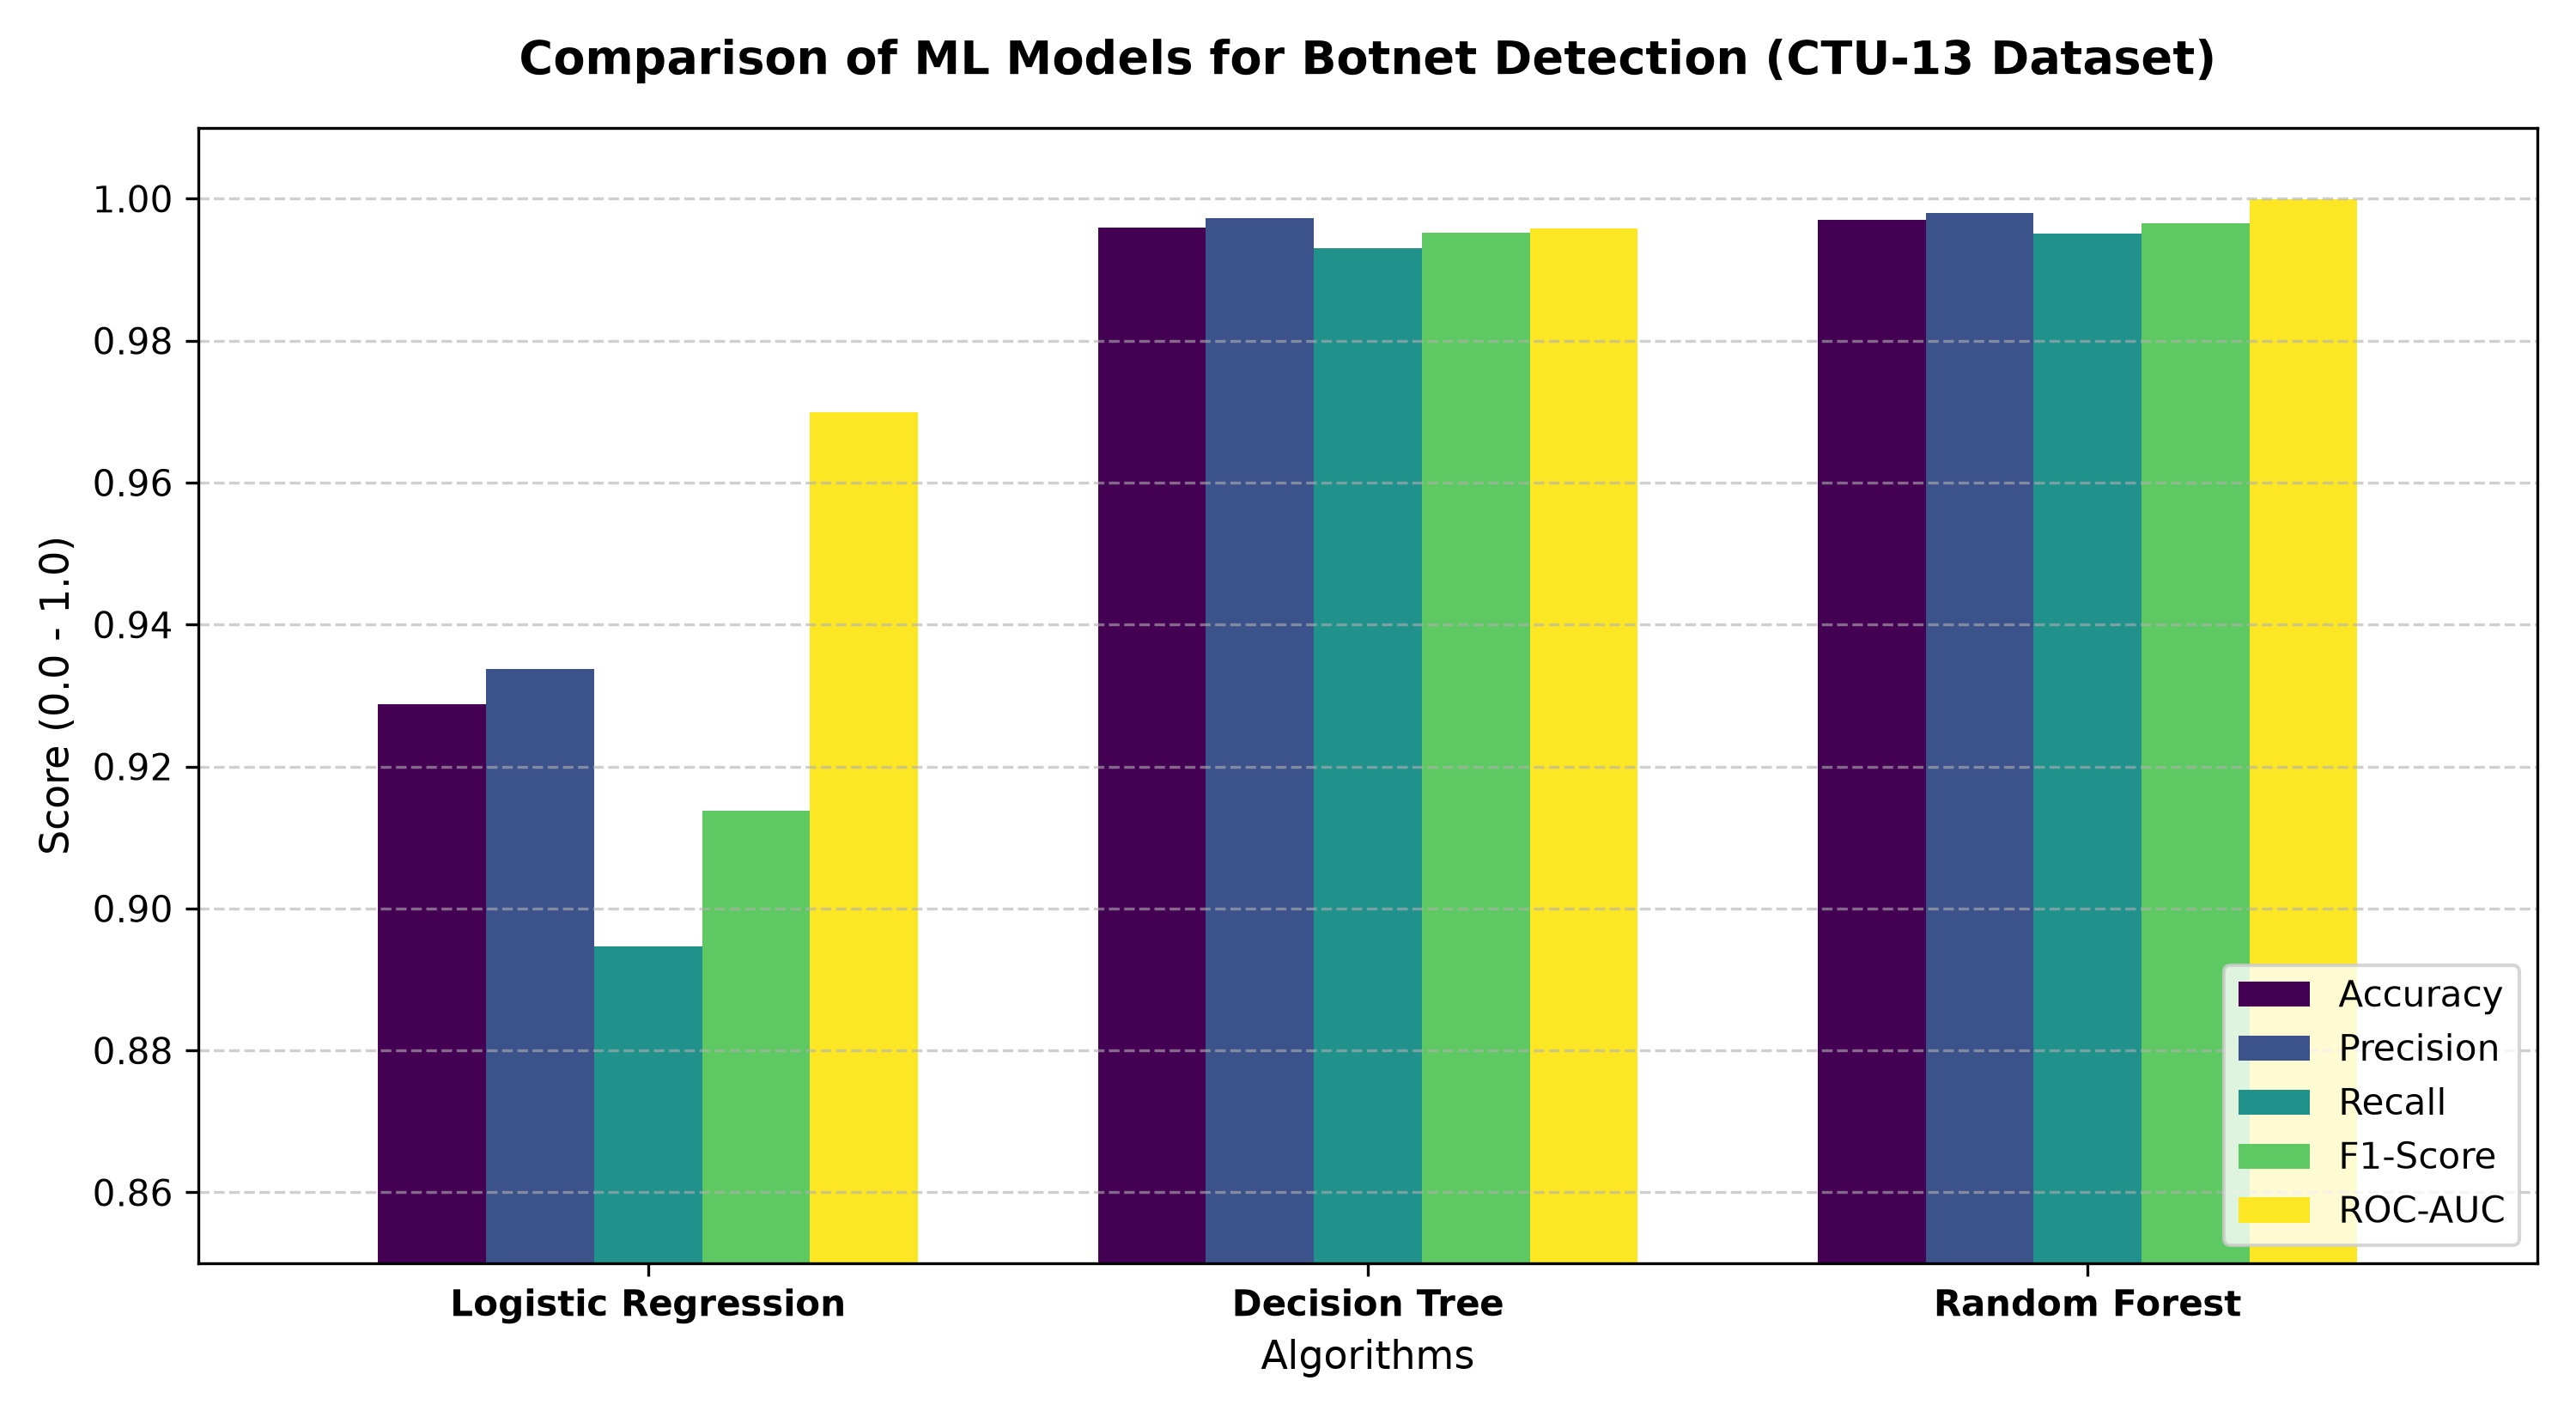
\includegraphics[width=0.75\textwidth, height=4.2cm]{1_metrics_comparison.png}
    }{
      \textit{(Xem biểu đồ tại output\_charts/1\_metrics\_comparison.png)}
    }
  \end{center}
\end{frame}

% SLIDE 7: MA TRẬN NHẦM LẪN & ROC CURVE
\begin{frame}{6. Đánh giá chi tiết mô hình Random Forest}
  \begin{columns}[c]
    \begin{column}{0.5\textwidth}
      \centering
      \textbf{Ma trận nhầm lẫn (Confusion Matrix)}
      \IfFileExists{2_confusion_matrix_rf.png}{
        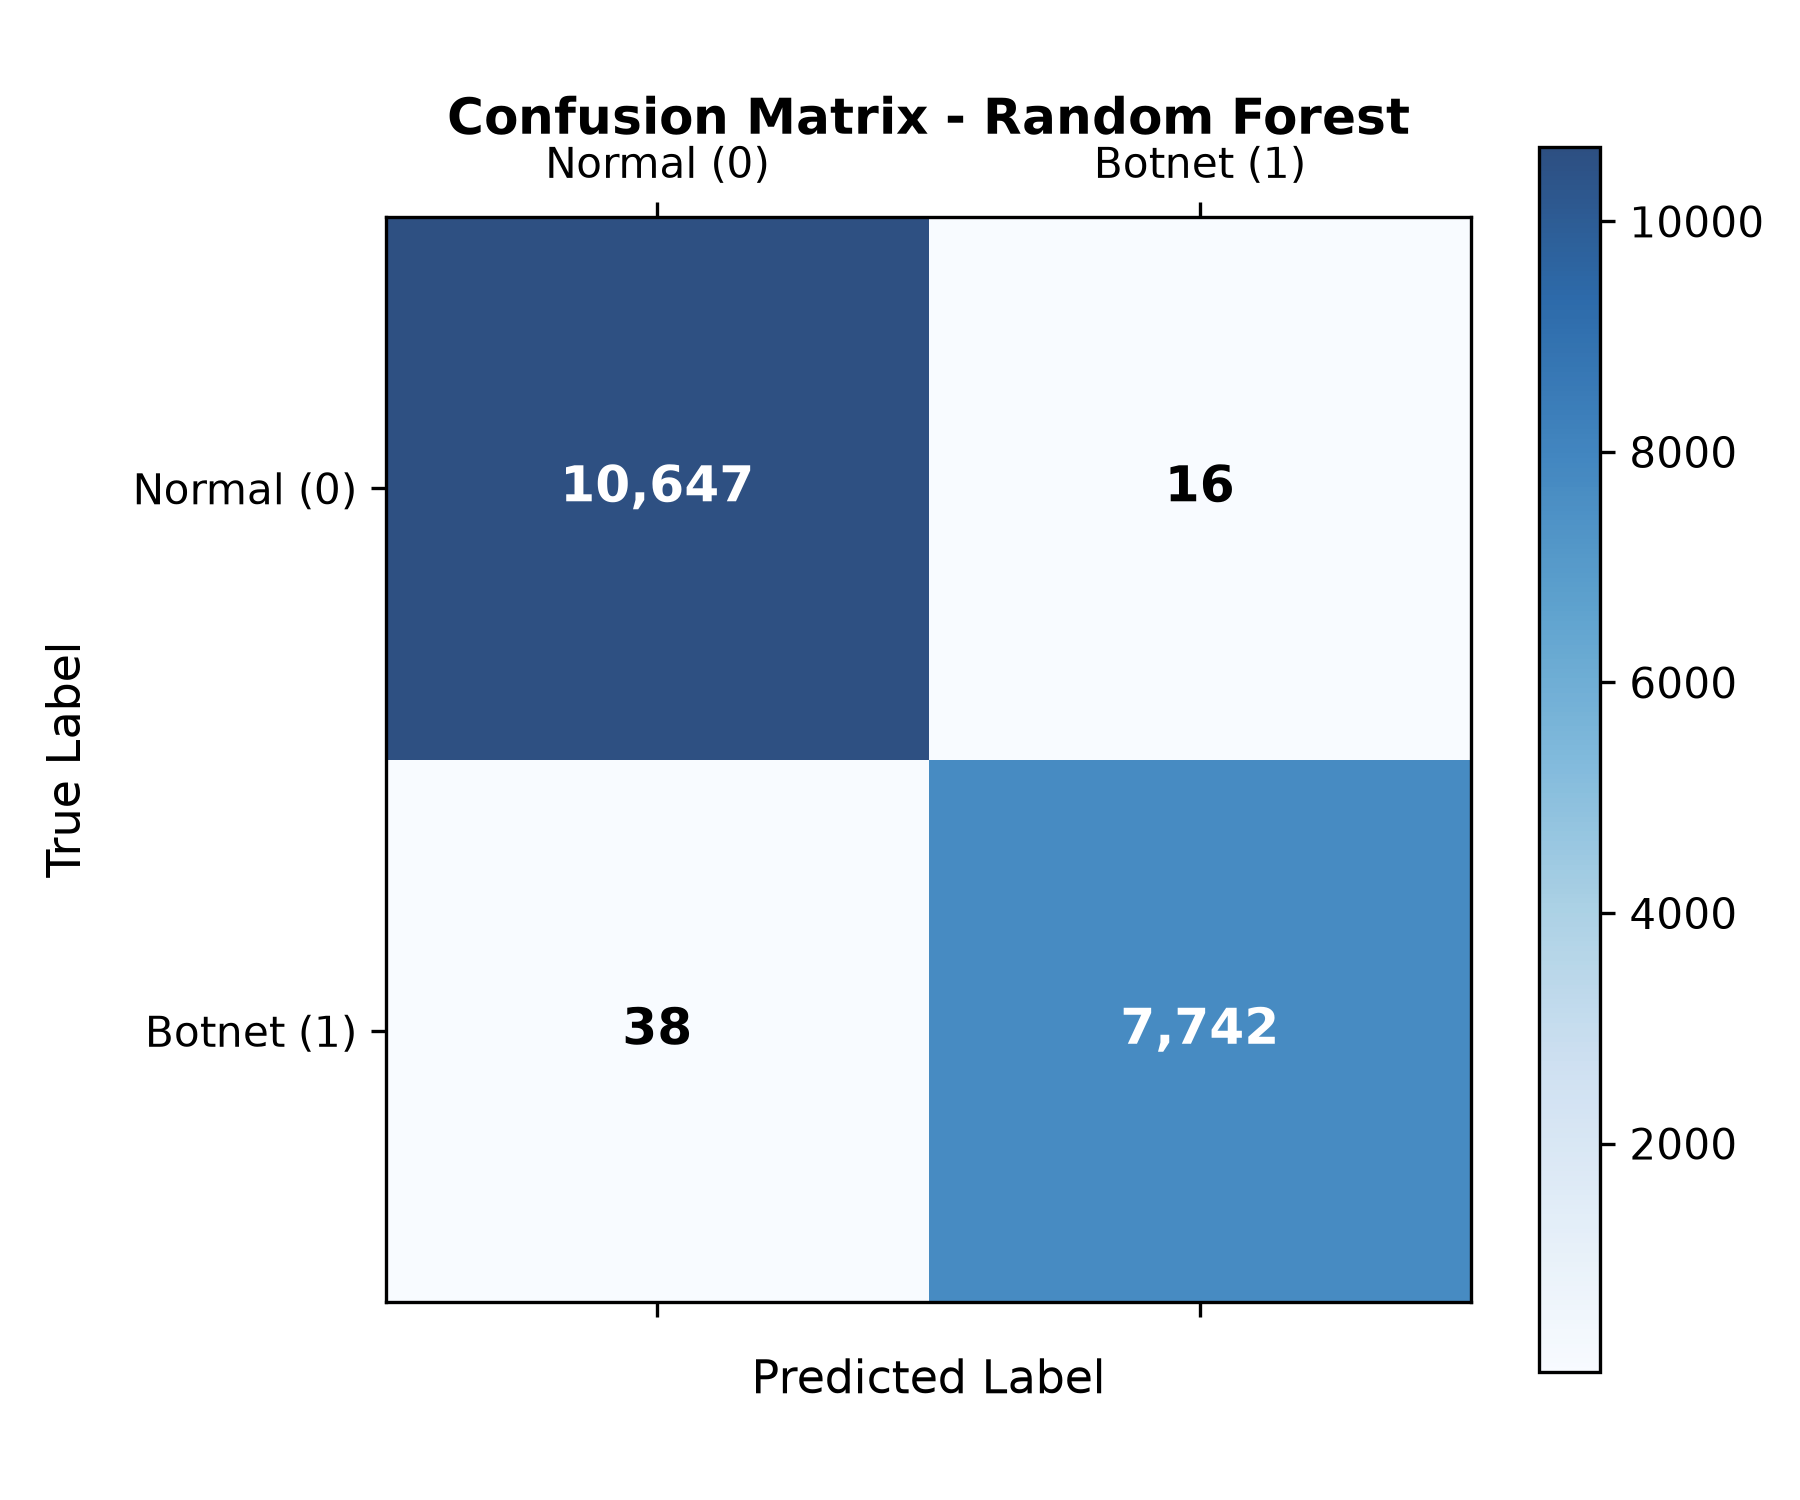
\includegraphics[width=\textwidth, height=4.3cm, keepaspectratio]{2_confusion_matrix_rf.png}
      }{}
      \begin{itemize}
        \item \textbf{Recall = 99.51\%:} Hầu như không bỏ lọt các luồng Botnet (False Negative cực thấp).
      \end{itemize}
    \end{column}
    \begin{column}{0.5\textwidth}
      \centering
      \textbf{Đường cong ROC (Receiver Operating)}
      \IfFileExists{3_roc_curves.png}{
        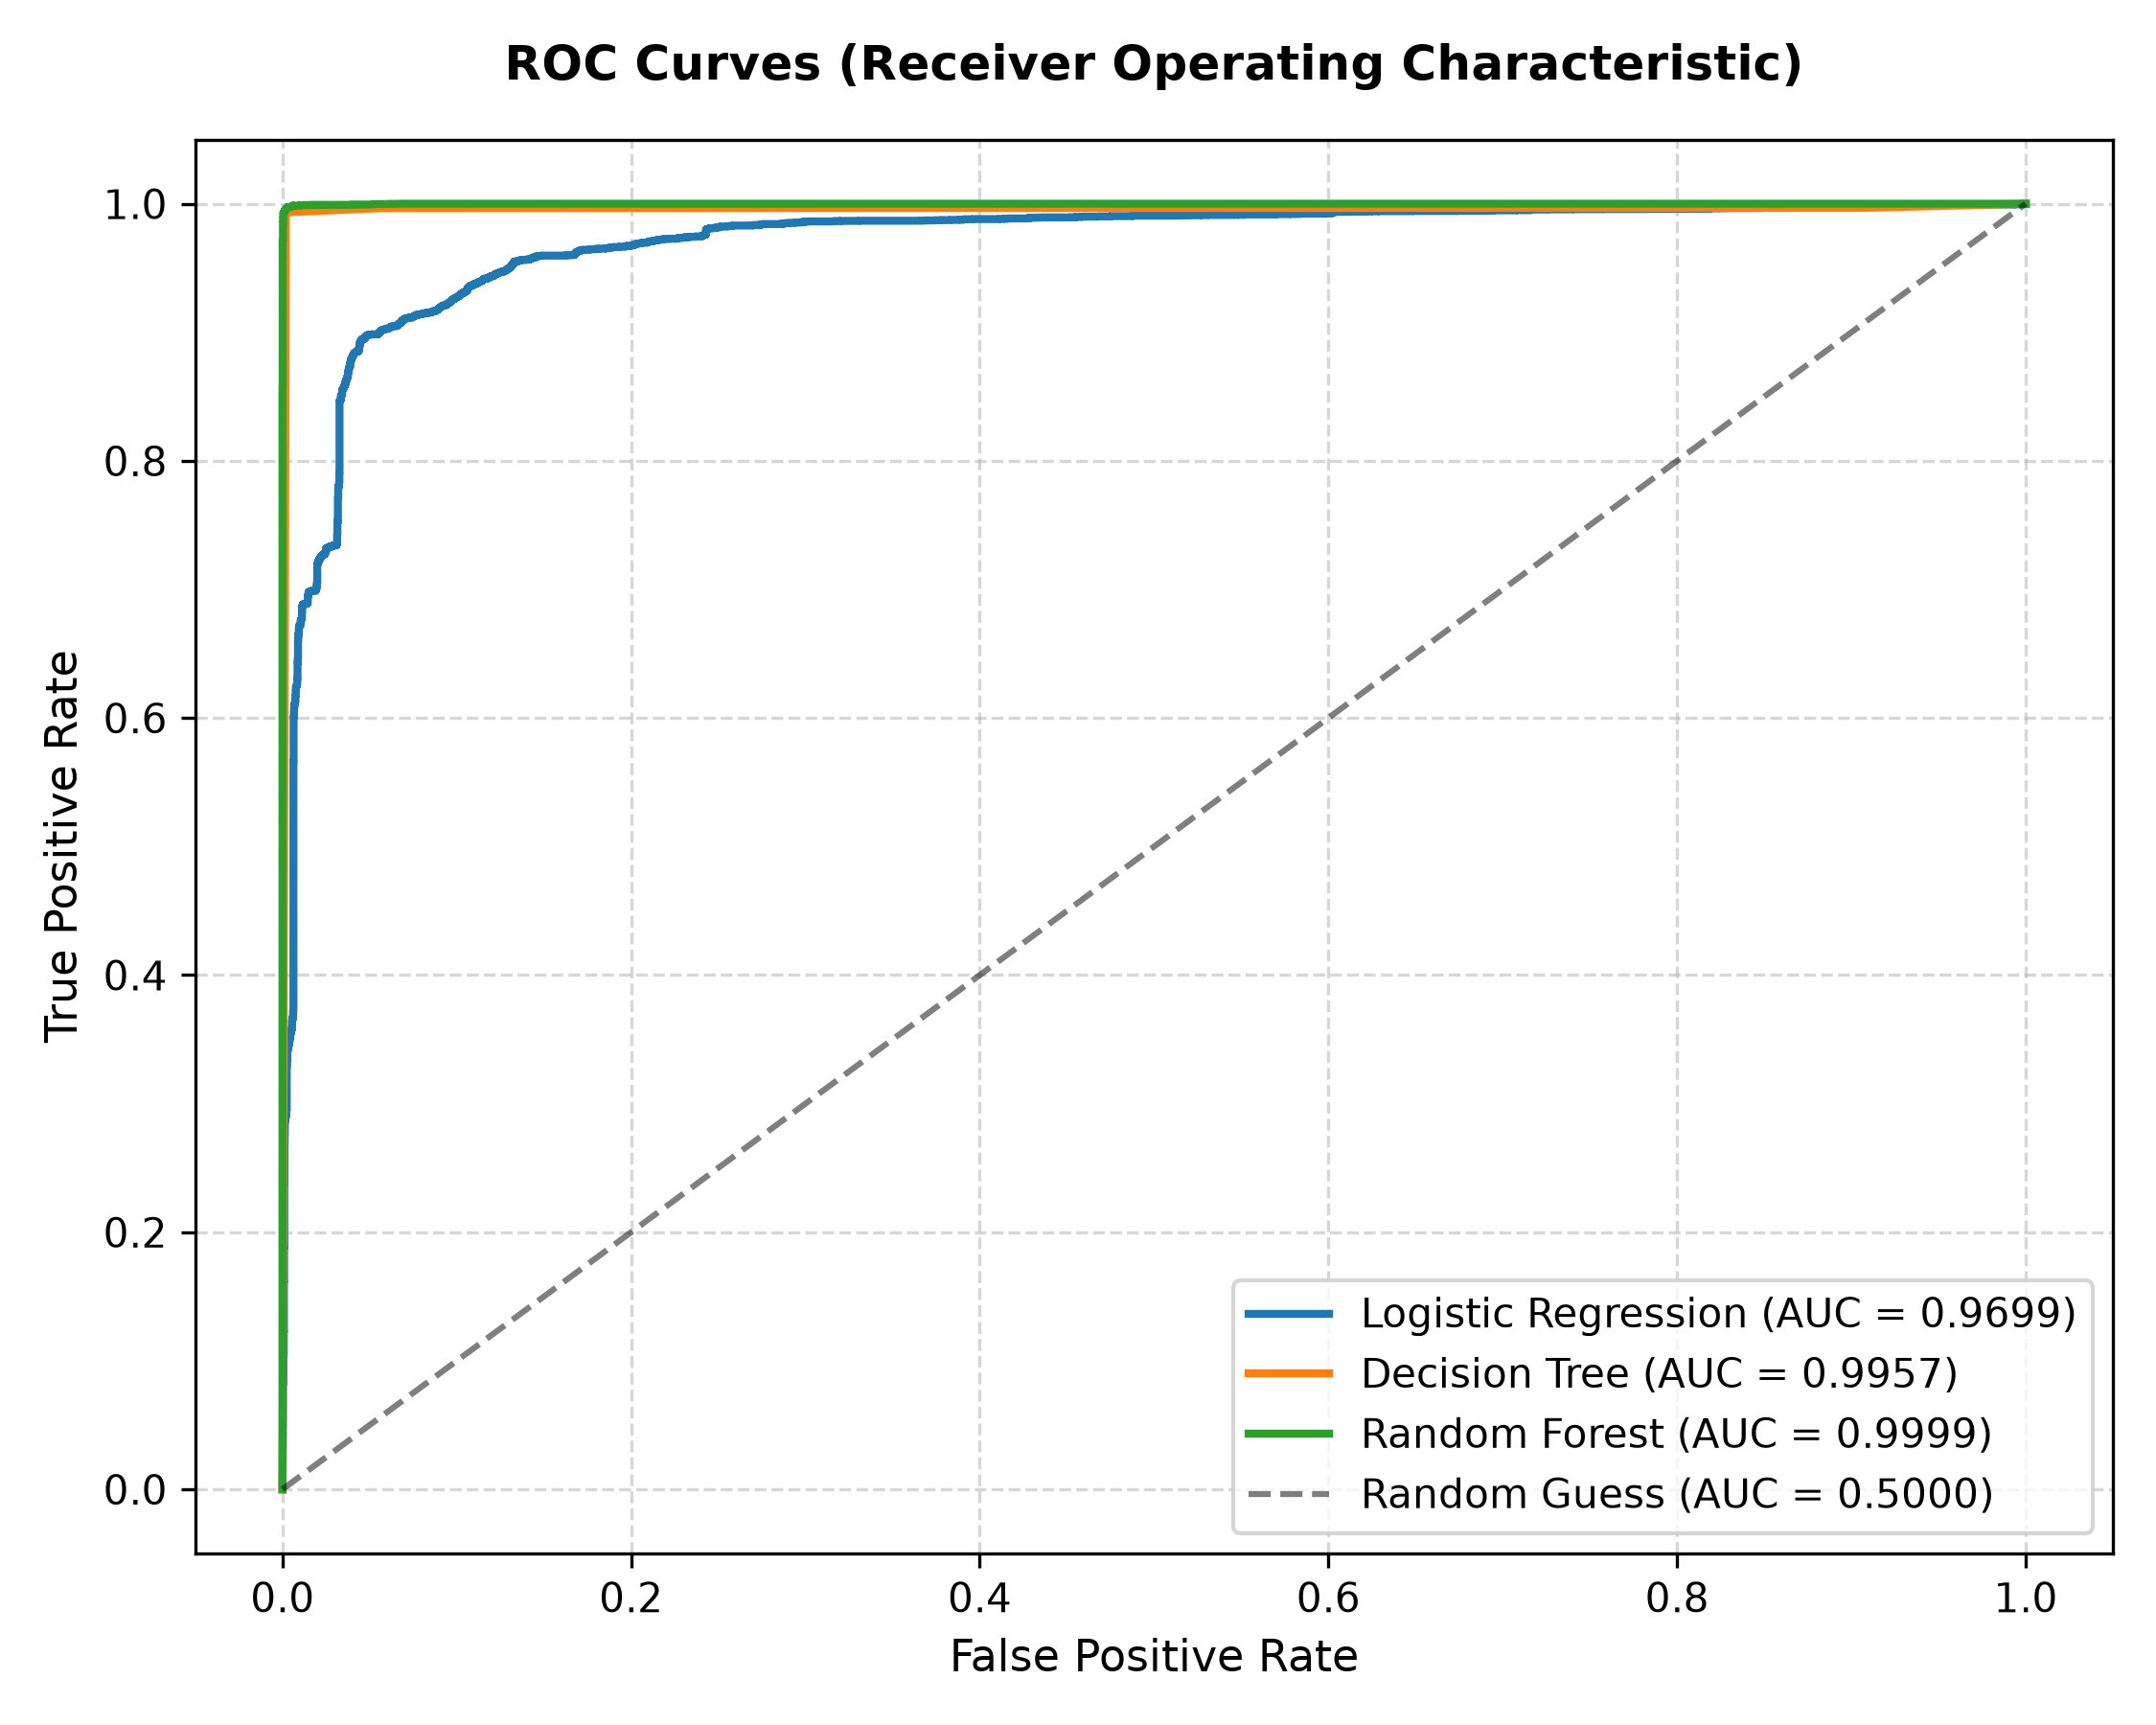
\includegraphics[width=\textwidth, height=4.3cm, keepaspectratio]{3_roc_curves.png}
      }{}
      \begin{itemize}
        \item \textbf{AUC = 0.9999:} Năng lực phân tách tuyệt đối giữa lưu lượng sạch và mã độc.
      \end{itemize}
    \end{column}
  \end{columns}
\end{frame}

% SLIDE 8: PHÂN TÍCH ĐẶC TRƯNG QUAN TRỌNG
\begin{frame}{7. Đóng góp đặc trưng (Feature Importance)}
  \begin{columns}[c]
    \begin{column}{0.58\textwidth}
      \IfFileExists{4_feature_importance_rf.png}{
        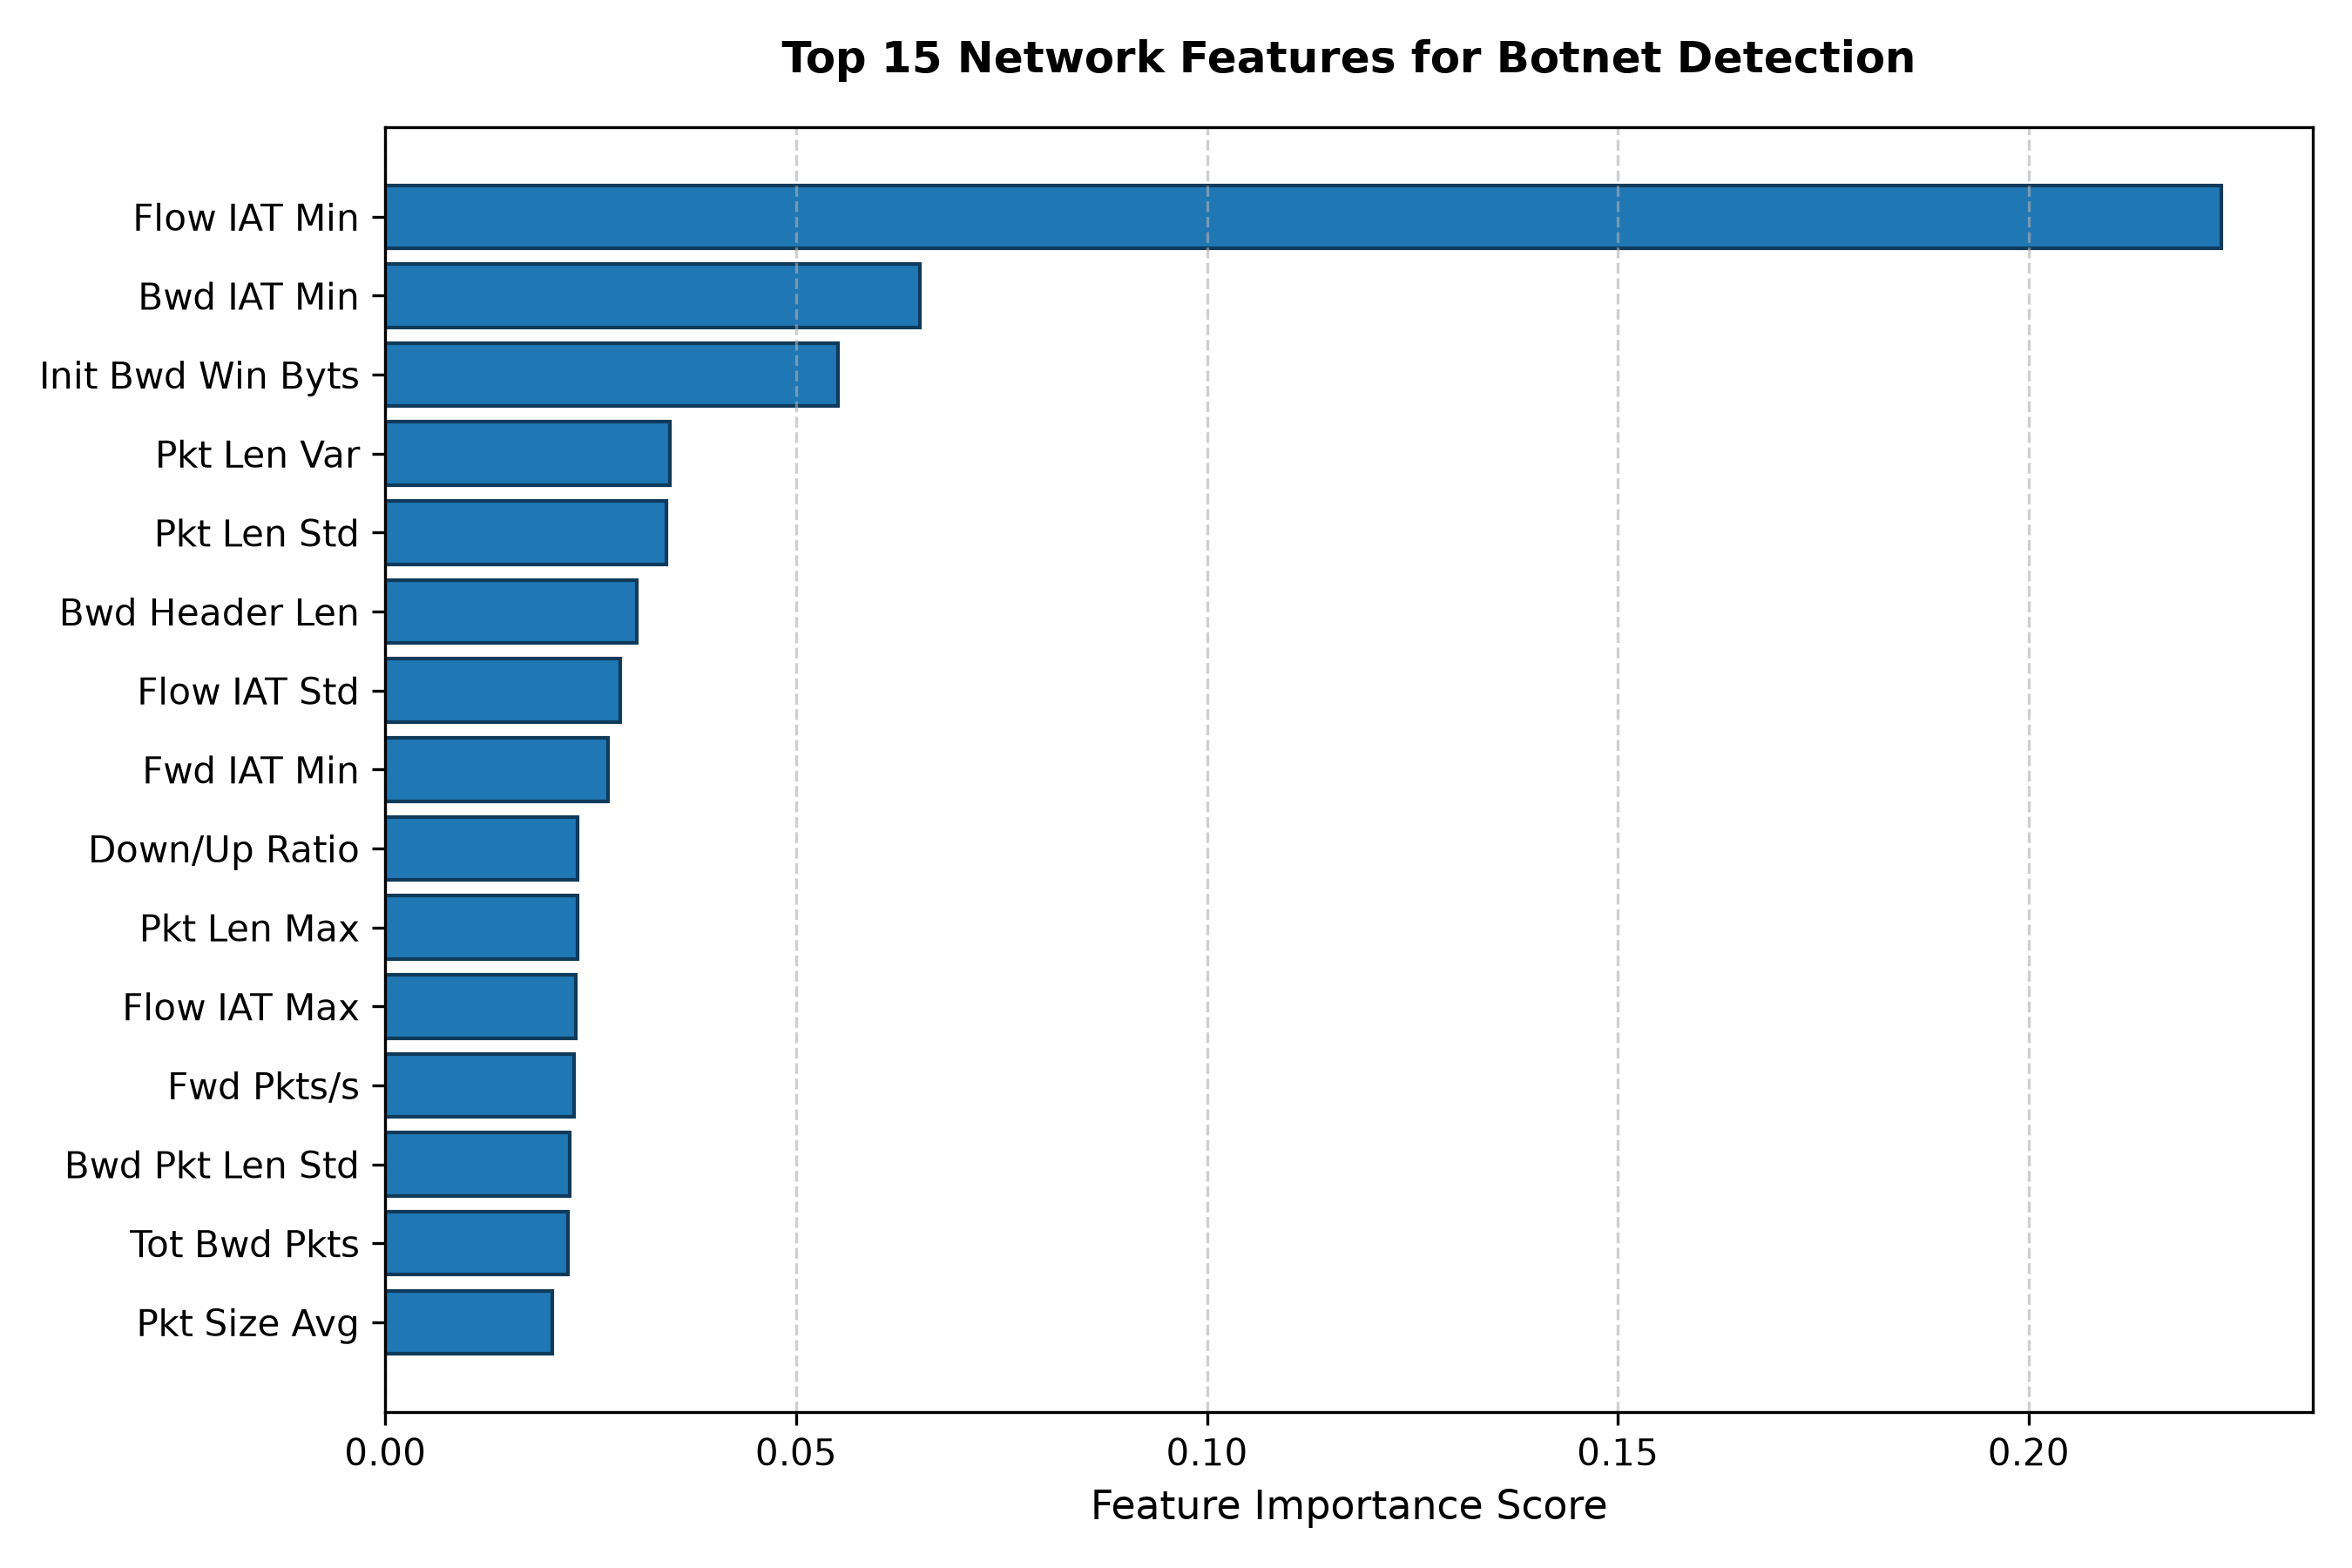
\includegraphics[width=\textwidth, height=5.2cm, keepaspectratio]{4_feature_importance_rf.png}
      }{}
    \end{column}
    \begin{column}{0.4\textwidth}
      \begin{block}{\textbf{Ý nghĩa An toàn thông tin}}
        \footnotesize
        \begin{itemize}
          \item \textbf{Flow IAT / Bwd IAT Min:} Khoảng cách giữa các gói tin thể hiện tốc độ phát tán tự động bằng script của botnet.
          \item \textbf{Pkt Len Var / Std:} Độ biến thiên kích thước gói; botnet có độ biến thiên rất thấp do dùng cấu trúc gói tin cố định.
          \item \textbf{Down/Up Ratio:} Đảo ngược hoàn toàn so với duyệt web thông thường.
        \end{itemize}
      \end{block}
    \end{column}
  \end{columns}
\end{frame}

% SLIDE 9: THỰC NGHIỆM MỞ RỘNG - LỰA CHỌN ĐẶC TRƯNG
\begin{frame}{8. Thực nghiệm mở rộng: Lựa chọn đặc trưng (Feature Selection)}
  \begin{block}{\textbf{Đặt bài toán thực tế cho thiết bị phần cứng}}
    Trong thực tế, tính toán cùng lúc 57 đặc trưng cho hàng triệu gói tin trên Router/Firewall sẽ gây quá tải CPU và trễ mạng. Nhóm thử nghiệm rút gọn xuống \textbf{Top 10 đặc trưng quan trọng nhất}.
  \end{block}

  \vspace{0.2cm}
  \begin{table}[h]
    \centering
    \small
    \begin{tabular}{lccc}
      \toprule
      \textbf{Tiêu chí} & \textbf{Dùng cả 57 đặc trưng} & \textbf{Top 10 đặc trưng} & \textbf{Hiệu quả tối ưu} \\
      \midrule
      \textbf{Số lượng đặc trưng} & 57 & \textbf{10} & \textbf{Giảm 82.5\%} \\
      \textbf{Độ chính xác (Accuracy)} & 99.89\% & \textbf{99.82\%} & \textit{Tương đương ($>99.8\%$)} \\
      \textbf{F1-Score} & 0.9965 & \textbf{0.9978} & \textit{Tối ưu hơn do bỏ nhiễu} \\
      \textbf{Thời gian suy luận Test} & 62.3 ms & \textbf{56.3 ms} & \textbf{Nhanh hơn $\approx 10\%$} \\
      \bottomrule
    \end{tabular}
  \end{table}

  \begin{exampleblock}{\textbf{Kết luận kỹ thuật}}
    Chỉ cần theo dõi 10 chỉ số luồng cốt lõi là đủ để bảo vệ hệ thống mạng với hiệu năng tối đa.
  \end{exampleblock}
\end{frame}

% SLIDE 10: DEMO THỰC TẾ & LIÊN HỆ SLIPS
\begin{frame}{9. Triển khai thực tế \& Liên hệ Stratosphere IPS (Slips)}
  \begin{columns}[T]
    \begin{column}{0.48\textwidth}
      \begin{block}{\textbf{Thực nghiệm Suy diễn trực tiếp}}
        \begin{itemize}
          \item Đóng gói mô hình thành công: \texttt{random\_forest\_botnet.pkl}.
          \item Xây dựng script \texttt{demo\_detect.py}: Nhận diện thời gian thực luồng mạng với độ trễ \textbf{$< 2$ms/flow}.
          \item Xác thực $100\%$ chính xác trên các mẫu luồng Botnet ngẫu nhiên.
        \end{itemize}
      \end{block}
    \end{column}
    \begin{column}{0.48\textwidth}
      \begin{block}{\textbf{Liên hệ hệ thống Slips (Stratosphere)}}
        \begin{itemize}
          \item Slips sử dụng Zeek để tạo luồng và mã hóa hành vi thành các trạng thái ký tự (Behavioral letters).
          \item Pipeline của nhóm đóng vai trò hạt nhân Machine Learning cốt lõi (tương đương module \texttt{flowmldetection} của Slips).
        \end{itemize}
      \end{block}
    \end{column}
  \end{columns}
\end{frame}

% SLIDE 11: KẾT LUẬN & HƯỚNG PHÁT TRIỂN
\begin{frame}{10. Kết luận \& Hướng phát triển}
  \begin{block}{\textbf{Kết quả đạt được}}
    \begin{enumerate}
      \item Xây dựng thành công pipeline trích xuất luồng và phân loại Botnet bằng Machine Learning.
      \item Mô hình Random Forest đạt độ chính xác \textbf{99.71\%}, Recall \textbf{99.51\%}, chứng minh tính ưu việt của phân tích luồng khi dữ liệu bị mã hóa.
      \item Chứng minh tính khả thi của việc tối ưu hóa đặc trưng (chỉ cần 10 đặc trưng vẫn giữ độ chính xác 99.82\%).
    \end{enumerate}
  \end{block}

  \vspace{0.2cm}
  \begin{alertblock}{\textbf{Hướng phát triển}}
    \begin{itemize}
      \item Khắc phục hiện tượng \textit{Flow Correlation} bằng cách đánh giá theo trục thời gian (\textit{Time-based split}).
      \item Thử nghiệm mô hình trên các họ Botnet biến thể mới chưa từng xuất hiện trong tập huấn luyện (Zero-day Botnet).
    \end{itemize}
  \end{alertblock}
\end{frame}

% SLIDE 12: CẢM ƠN & HỎI ĐÁP
\begin{frame}[plain]
  \begin{center}
    \vspace{1cm}
    \IfFileExists{logo_huce.png}{
      
\includegraphics[height=1.8cm]{logo_huce.png}
    }{}
    
    \vspace{0.5cm}
    {\LARGE \textbf{\color{HuceBlue} XIN TRÂN TRỌNG CẢM ƠN!}}
    
    \vspace{0.3cm}
    {\large Quý Thầy/Cô và Hội đồng đánh giá}
    
    \vspace{0.8cm}
    \textbf{Q \& A: SẴN SÀNG TRẢ LỜI CÂU HỎI PHẢN BIỆN}
  \end{center}
\end{frame}

\end{document}
